\siFigure{../../images/grid-bathymetry-map.pdf}{
    \jroeditnoteb{New figure.}
    \jroeditb{}{%
    Bathymetry contours around the Philippine Islands at varying depths.
    Black lines show the contour associated with the depth indicated
    in the upper right of each plot.
    Contours are based on data from the ETOPO1 1-arc-minute global relief model
    \citep{Amante2009}.
    Figure generated with marmap version 1.0.2 \citep{Pante2013} and ggplot2
    Version 2.2.1 \citep{ggplot2}.}
}{fig:bathycontours}

\begin{figure}[htbp]
\begin{center}
    \includemedia[
        % width=0.8\linewidth,
        height=0.8\textheight,
        activate=pagevisible,
        deactivate=pageinvisible,
        passcontext,
        transparent=false,
        addresource=../../images/bathymetry-maps/animated-bathymetry.mp4,
        flashvars={source=../../images/bathymetry-maps/animated-bathymetry.mp4}
    ]{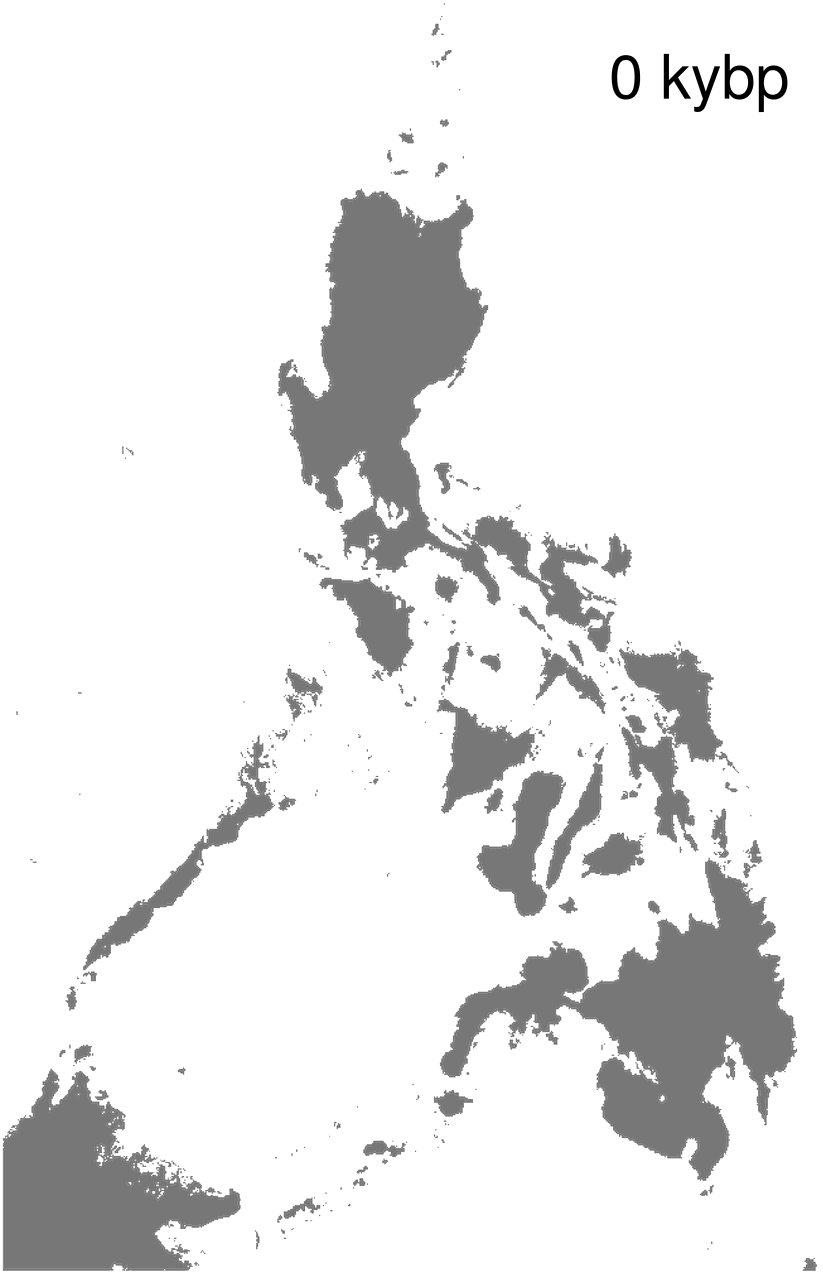
\includegraphics[height=0.8\textheight]{../../images/bathymetry-maps/animated-bathymetry-last-frame.png}}{VPlayer.swf}
    \captionsetup{name=Figure S, labelformat=noSpace, listformat=sFigList}
    \caption{
        \jroeditnoteb{New figure.}
        \jroeditb{}{%
        Animation of approximate sea-level changes in the Philippine Islands
        over the last 430,000 years.
        Sea-level estimates are from the projection of \citet{Spratt2016} based
        on seven reconstructions.
        Bathymetry data are from the ETOPO1 1-arc-minute global relief model
        \citep{Amante2009}.
        Animation generated using marmap version 1.0.2 \citep{Pante2013},
        ggplot2
        Version 2.2.1 \citep{ggplot2},
        \href{https://imagemagick.org/index.php}{ImageMagick}
        Version 6.9.10-8 Q16 x86\_64 20180723,
        and \href{https://ffmpeg.org/}{FFmpeg}
        Version 4.0.2-2.
        The source code for generating the plot is available at
        \url{https://github.com/phyletica/animating-sea-level-change}.
        This animation can also be viewed at
        \url{https://youtu.be/NjGdCezUvw8}.}
    }
    \label{fig:bathyanimation}
\end{center}
\end{figure}

\siFigure{../../../data/genomes/msg/ecoevolity-results/grid-cyrtodactylus-sumevents.pdf}{
    Approximate prior (light bars) and posterior (dark bars) probabilities
    of numbers of divergence events across pairs of \spp{Cyrtodactylus}
    populations
    under three different priors on the concentration parameter of
    the Dirichlet process.
    Bayes factors for each number of divergence times is given above the
    corresponding bars.
    Each Bayes factor compares the corresponding number of events 
    to all other possible numbers of divergence events.
    \weusedggplot
}{fig:cyrtneventsbyconcentration}

\siFigure{../../../data/genomes/msg/ecoevolity-results/grid-cyrtodactylus-sumtimes.pdf}{
    Approximate marginal posterior densities of divergence times for each
    pair of \spp{Cyrtodactylus} populations
    under three different priors on the concentration parameter of
    the Dirichlet process.
    \weusedggridges
}{fig:cyrtdivtimesbyconcentration}

\siFigure{../../../data/genomes/msg/ecoevolity-results/grid-cyrtodactylus-sumevents-nopoly.pdf}{
    Approximate prior (light bars) and posterior (dark bars) probabilities
    of numbers of divergence events across pairs of \spp{Cyrtodactylus}
    populations
    under four different combinations of prior on divergence times (rows)
    and recoding or removing polyallelic characters (columns).
    Bayes factors for each number of divergence times is given above the
    corresponding bars.
    Each Bayes factor compares the corresponding number of events 
    to all other possible numbers of divergence events.
    \weusedggplot
}{fig:cyrtneventsbytimeprior}

\siFigure{../../../data/genomes/msg/ecoevolity-results/grid-cyrtodactylus-sumtimes-nopoly.pdf}{
    Approximate marginal posterior densities of divergence times for each
    pair of \spp{Cyrtodactylus} populations
    under four different combinations of prior on divergence times (rows)
    and recoding or removing polyallelic characters (columns).
    \weusedggridges
}{fig:cyrtdivtimesbytimeprior}



\siFigure{../../../data/genomes/msg/ecoevolity-results/grid-cyrtodactylus-sumsizes.pdf}{
    Approximate marginal posterior densities of population sizes for each
    pair of \spp{Cyrtodactylus} populations
    under three different priors on the concentration parameter of
    the Dirichlet process.
    \weusedggridges
}{fig:cyrtpopsizesbyconcentration}

\siFigure{../../../data/genomes/msg/ecoevolity-results/grid-cyrtodactylus-sumsizes-nopoly.pdf}{
    Approximate marginal posterior densities of population sizes for each
    pair of \spp{Cyrtodactylus} populations
    under four different combinations of prior on divergence times (rows)
    and recoding or removing polyallelic characters (columns).
    \weusedggridges
}{fig:cyrtpopsizesbytimeprior}



\siFigure{../../../data/genomes/msg/ecoevolity-results/grid-gekko-sumevents.pdf}{
    Approximate prior (light bars) and posterior (dark bars) probabilities
    of numbers of divergence events across pairs of \spp{Gekko}
    populations
    under three different priors on the concentration parameter of
    the Dirichlet process.
    Bayes factors for each number of divergence times is given above the
    corresponding bars.
    Each Bayes factor compares the corresponding number of events 
    to all other possible numbers of divergence events.
    \weusedggplot
}{fig:gekkoneventsbyconcentration}

\siFigure{../../../data/genomes/msg/ecoevolity-results/grid-gekko-sumtimes.pdf}{
    Approximate marginal posterior densities of divergence times for each
    pair of \spp{Gekko} populations
    under three different priors on the concentration parameter of
    the Dirichlet process.
    \weusedggridges
}{fig:gekkodivtimesbyconcentration}

\siFigure{../../../data/genomes/msg/ecoevolity-results/grid-gekko-sumevents-nopoly.pdf}{
    Approximate prior (light bars) and posterior (dark bars) probabilities
    of numbers of divergence events across pairs of \spp{Gekko}
    populations
    under six different combinations of prior on divergence times (rows)
    and recoding or removing polyallelic characters (columns).
    Bayes factors for each number of divergence times is given above the
    corresponding bars.
    Each Bayes factor compares the corresponding number of events 
    to all other possible numbers of divergence events.
    \weusedggplot
}{fig:gekkoneventsbytimeprior}

\siFigure{../../../data/genomes/msg/ecoevolity-results/grid-gekko-sumtimes-nopoly.pdf}{
    Approximate marginal posterior densities of divergence times for each
    pair of \spp{Gekko} populations
    under six different combinations of prior on divergence times (rows)
    and recoding or removing polyallelic characters (columns).
    \weusedggridges
}{fig:gekkodivtimesbytimeprior}


\siFigure{../../../data/genomes/msg/ecoevolity-results/grid-gekko-sumsizes.pdf}{
    Approximate marginal posterior densities of population sizes for each
    pair of \spp{Gekko} populations
    under three different priors on the concentration parameter of
    the Dirichlet process.
    \weusedggridges
}{fig:gekkopopsizesbyconcentration}

\siFigure{../../../data/genomes/msg/ecoevolity-results/grid-gekko-sumsizes-nopoly.pdf}{
    Approximate marginal posterior densities of population sizes for each
    pair of \spp{Gekko} populations
    under six different combinations of prior on divergence times (rows)
    and recoding or removing polyallelic characters (columns).
    \weusedggridges
}{fig:gekkopopsizesbytimeprior}

\siFigure{../../../data/genomes/msg/ecoevolity-simulations/plots/ancestor-size-scatter.pdf}{
    \jroeditnote{New figure.}
    \jroedit{}{%
    The accuracy and precision of \ecoevolity estimates of the ancestral
    population size (scaled by the mutation rate) when applied to data
    simulated to match our \spp{Cyrtodactylus} (left) and \spp{Gekko} (right)
    RADseq \datasets with all sites (top) or only one SNP per locus (bottom).
    Each circle and associated error bars represent the posterior mean
    and 95\% credible interval.
    Estimates for which the potential-scale reduction factor
    % Details of the PSRF calculation are in the main text, so we
    % don't need this
    % \citep[PSRF; the square root of Equation 1.1 in][]{Brooks1998}
    was greater than 1.2
    \citep{Brooks1998} are highlighted in orange.
    Each plot consists of 4000 estimates---500 simulated \datasets, each with
    eight pairs of populations.
    For each plot, the root-mean-square error (RMSE) and the proportion of
    estimates for which the 95\% credible interval contained the true
    value---$p(\epopsize{}\murate{} \in \textrm{CI})$---is given.
    \weusedmatplotlib}
}{fig:simsancestralsizes}

\siFigure{../../../data/genomes/msg/ecoevolity-simulations/plots/descendant-size-scatter.pdf}{
    \jroeditnote{New figure.}
    \jroedit{}{%
    Accuracy and precision of \ecoevolity estimates of the descendant
    population sizes (scaled by the mutation rate) when applied to data
    simulated to match empirical \spp{Cyrtodactylus} (left) and \spp{Gekko} (right)
    RADseq \datasets with all sites (top) or only one SNP per locus (bottom).
    Each circle and associated error bars represents the posterior mean
    and 95\% credible interval.
    Estimates for which the potential-scale reduction factor
    % Details of the PSRF calculation are in the main text, so we
    % don't need this
    % \citep[PSRF; the square root of Equation 1.1 in][]{Brooks1998}
    was greater than 1.2
    \citep{Brooks1998} are highlighted in orange.
    Each plot consists of 8000 estimates---500 simulated \datasets, each with
    eight pairs of populations.
    For each plot, the root-mean-square error (RMSE) and the proportion of
    estimates for which the 95\% credible interval contained the true
    value---$p(\epopsize{}\murate{} \in \textrm{CI})$---is given.
    \weusedmatplotlib}
}{fig:simsdescendantsizes}

\siFigure{../../../data/genomes/msg/ecoevolity-simulations/plots/cyrt-event-time-sampling-disparity-scatter.pdf}{
    \jroeditnote{New figure.}
    \jroedit{}{%
    Accuracy and precision of \ecoevolity divergence-time estimates (in units
    of expected subsitutions per site) when applied to data simulated to match
    empirical RADseq \datasets sampled from the pairs of \spp{Cyrtodactylus
        philippinicus} populations from the islands of (left) Luzon and Babuyan
    Claro and (right) Polillo and Luzon
    (a subset of the results plotted in Figure~\ref{fig:simsdivtimes}).
    Results are shown for \ecoevolity analyses of \datasets that contain all
    sites (top), or only one SNP per locus (bottom).
    The number of individuals sampled from each island population is indicated
    in \jroeditb{parantheses}{parentheses} at the top of each column of plots.
    Results for these two pairs of populations are plotted separately here to
    compare divergence-times estimated from \datasets with large differences in
    the number of sampled individuals and loci.
    Each circle and associated error bars represents the posterior mean and 95\%
    credible interval for the time that a pair of populations diverged.
    Estimates for which the potential-scale reduction factor
    % Details of the PSRF calculation are in the main text, so we
    % don't need this
    % \citep[PSRF; the square root of Equation 1.1 in][]{Brooks1998}
    was greater than 1.2
    \citep{Brooks1998} are highlighted in orange.
    Each plot consists of 500 estimates---one from each of the 500 simulated
    \datasets.
    For each plot, the root-mean-square error (RMSE) and the proportion of
    estimates for which the 95\% credible interval contained the true
    value---$p(\comparisondivtime{} \in \textrm{CI})$---is given.
    \weusedmatplotlib}
}{fig:sampledisparitydivtimes}
